% PROTOKOLL Action Item
\documentclass[
   draft=false
  ,paper=a4
  ,twoside=false
  ,fontsize=11pt
  ,headsepline
  ,DIV=11
  ,parskip=full+
  ,titlepage
]{scrartcl} % copied from Thesis Template from HAW

\usepackage[ngerman,english]{babel}

\usepackage[T1]{fontenc}
\usepackage[utf8]{inputenc}

\usepackage[
    left  =4em
   ,right =4em
   ,top   =5em
   ,bottom=5em
]{geometry}

\usepackage{longtable}
\usepackage[german,refpage]{nomencl}

\usepackage{float}
%\usepackage{enumitem}
\usepackage{paralist} %compactitem
\usepackage{graphicx}
%\usepackage{url}



\usepackage{hyperref} % for a better experience

\hypersetup{
   colorlinks=true % if false - links get colored frames
  ,linkcolor=black % color of tex intern links
  ,urlcolor=blue   % color of url links
  ,citecolor=black
}

\usepackage{amsmath}

\usepackage{array}   % for \newcolumntype macro
\newcolumntype{L}{>{$}l<{$}} % math-mode version of "l" column type
\newcolumntype{R}{>{$}r<{$}} % math-mode version of "r" column type
\newcolumntype{C}{>{$}c<{$}} % math-mode version of "c" column type

\usepackage{color}
\definecolor{black}{rgb}{0,0,0}
\definecolor{darkgray}{rgb}{0.2,0.2,0.2}
\definecolor{lightgray}{rgb}{0.9,0.9,0.9}
\definecolor{blue}{rgb}{0.0,0.0,0.9}
\definecolor{orange}{rgb}{0.7,0.3,0.0}
\definecolor{green}{rgb}{0.0,0.7,0.0}
\definecolor{red}{rgb}{0.9,0.0,0.0}

\usepackage{listings, lstautogobble}
\lstset{%
   language=bash
  ,frame=single
  ,numbers=left
  ,numberstyle=\tiny\color{darkgray}
  ,stepnumber=1
  ,numbersep=5pt
  ,backgroundcolor=\color{lightgray}
  ,showspaces=false
  ,keepspaces=true
  ,autogobble=true 
  ,breaklines=true
  ,tabsize=2
  , 
  ,basicstyle=\footnotesize\ttfamily\color{black}
  ,identifierstyle=\color{black}
  ,keywordstyle=[1]\color{blue}\textbf
  ,keywordstyle=[2]\color{red}\textbf
  ,stringstyle=\color{green}
  ,commentstyle=\color{darkgray}\textit
}
  
\usepackage{caption}
\usepackage{colortbl}
\definecolor{tabgrey}{rgb}{0.85,0.85,0.85}
%using minted because of the hashtag in bash

\sloppy
\clubpenalty=10000
\widowpenalty=10000
\displaywidowpenalty=10000


\usepackage{filecontents}

\usepackage{natbib}



% set font 
%\renewcommand{\familydefault}{\sfdefault}
\usepackage{times}

\begin{document}

\selectlanguage{ngerman}
% ----------------------------------------------------------------------------
% ---------------------------------------------------------- HIER WAS MACHEN -
% -------------------------------- Metadaten wie namen und Gruppentreffen etc-
\title{}
\subtitle{a git survival kit - german version}
\author{Martin Witte}
\author{%
        Martin Witte 
        \\ Karl-Fabian Witte
       }
\date{\today}

\publishers{%
	\normalfont\normalsize%
	\parbox{0.8\linewidth}{\centering
	  Dieses Dokument ist speziell für das Praktikum des ESE 
	  Moduls 2017 des Studienganges Technische Informatik der HAW Hamburg
	  erstellt worden und dient der Zusamenarbeit der Gruppe LANKE. 
		Es werden hier die Grundideen mit dem Umgang mit git und
		dem \"{}flow\"{} erklärt. Die Commit Message Struktur sowie die 
		Branchstruktur wird hier beschlossen. 
	}
}

\maketitle
\setcounter{page}{1}
\tableofcontents
\flushleft




\section{Verbesserungskonzept}




\section{Messung}

\begin{figure}[htp]
  \centering
  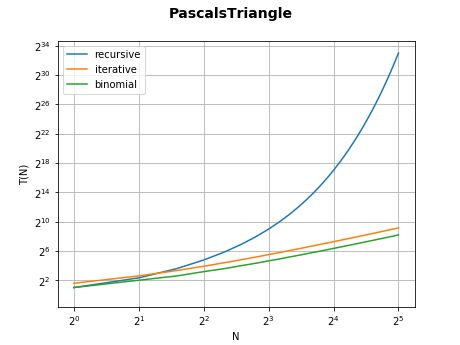
\includegraphics[width=\textwidth]{../sample.png}
  \caption[sample]{sample}
  \label{fig:sample}
\end{figure}



\begin{filecontents}{doc.bib}
@book{ProGit
  ,author    = {Chacon, Scott and Straub, Ben}
  ,title     = {Pro Git}
  ,year      = {2014}
  ,isbn      = {1484200772, 9781484200773}
  ,edition   = {2nd}
  ,publisher = {Apress}
  ,address   = {Berkely, CA, USA}
  ,note      = {\url{https://git-scm.com/book/en/v2} (2017-04-28)}
}

@misc{AngularJS
  ,author = {AngularJS}
  ,title  = {Contributing to {A}ngular{JS}}
  ,year   = {2017}
  ,howpublished = {\url{https://github.com/angular/angular.js/blob/master/CONTRIBUTING.md#commit} (2017-04-28)}
}
\end{filecontents}
	
	
\bibliographystyle{plainnat}
\bibliography{git.bib}
\end{document}